%%%%%%%%%%%%%%%%%%%%%%%%%%%%%%%%%%%%%%%%%%%%%%%%%%%%%%%%%%%%%%%%%%%%%%%%%%%%
\section{Supporting Information Appendix} \label{ap_a_dom_wells}

\subsection{Study Area}
\label{ap_a_study_area}

The study area was pared down from the Central Valley (CV) to only the area where more recently completed domestic wells (1976 and younger) were present. This cutoff was chosen because the model period in this study ends in 2016, thus wells completed on or after 1976 ($n = 67,011$) assumes a conservatively high well retirement age of 40 years. Circular, 5 $km$ buffers were drawn around each well, then joined to create a unified study area polygon. Some isolated circles that were not connected to any other buffers ($<$ 1\% of the buffered area) were removed in order to constrain the study site to one contiguous spatial extent in the CV corresponding to the areas of greatest domestic well density. The small removed areas principally occur in the western San Joaquin Valley. Low rates of domestic well completion in the west side of the San Joaquin Valley compared to the CV as a whole are explained by a relatively deep water table, poor shallow groundwater quality, and perhaps missing well completion records in places where there are actually households on unregistered or non-permitted domestic wells. 


%%%%%%%%%%%%%%%%%%%%%%%%%%%%%%%%
\subsection{Data}
\label{ap_a_data}

The California DWR keeps paper records of wells drilled in California that contain well construction information, such as the depth of the well, perforated interval dimensions, location, and well type (e.g. - irrigation, domestic, monitoring, etc.) among other data. These records are submitted by the well-drilling company to the state in the form of a Well Completion Report (WCR). Nearly all WCRs in the state have been digitally scanned, and key fields in the reports have been digitized. Until recently, WCR information was confidential under state law, and they were unavailable to the general public, limiting researchers' abilities to answer questions like those set forth in this study.

The State’s Household Water Supply Shortage Reporting System (HWSSRS) was established in late 2014 as a tool to capture information on water supplies running dry due to worsening drought conditions across California. The data gathered by the system was used for coordinating the State’s drought emergency response efforts.  The system was set up as a voluntary, self-reporting system and, as such, only represents some fraction of the actual water supply shortages occurring. Most of the reported shortages were dry wells, but some were streams. Most of the reports were actually received by county health officials who entered the data into the system. Some counties were very active in reporting, while some were not. A download of the reported HWSSRS data has been made available to researchers with redaction of some data fields and a reduction in the accuracy of geospatial data to protect personal identification. The precision of the geospatial data is 36 arc seconds, corresponding to approximately 1 $km$ in the study area. The coordinate reference system used in this study is EPSG 4326.  

The great majority of well locations in OSCWR ($>$ 95\%) are rounded to the nearest centroid of the Public Land Survey System (PLSS) section. The PLSS is composed of a nested series of cadastral surveyed lands (e.g. townships, range and sections). Townships measure 6x6 square miles (93.24 $km^2$ each) in size and are made up of thirty-six one-square mile sections (2.56 $km^2$). As the distance between the cell centroid and a corner of each section is the half-diagonal $0.5\cdot\sqrt{2}\cdot1.6 = 1.14$ $km$, the reported location \textit{(x, y)} of each well is always 0 $\leq$ \textit{(x, y)}  $\leq 1.14$ $km$ from the true location. Determining the exact location of a well from the scanned well completion reports is intractable as well coordinates are rarely provided on the scanned forms, and the listed street address typically corresponds to the well owner's residence, not necessarily where the well is located, thus hampering efforts at geocoding. Due to these limitations, the reported PLSS section centroid was taken as the approximate well location, with a maximum error of 1.14 $km$.

%%%%%%%%%%%%%%%%%%%%%%%%%%%%%%%%
\subsection{Formal evaluation of well failure}
\label{ap_a_formal_wf}

Classification into active wells and failing wells proceeds through several steps (Figure \ref{fig:tree}). Consider a well $i$. It has a set of spatial coordinates and an associated estimated pump depth $(x_i,y_i,z_i)$, where $x_i$ and $y_i$ are the Cartesian coordinates, and $z_i$ is the estimated depth of the pump within the well casing that draws water from the surrounding aquifer. The groundwater level $g$ is a scalar field which varies by location; the groundwater level at a well is thus a scalar defined by its coordinates: $g_i = f(x_i,y_i)$. We determine the groundwater level for some initial time $g({t_0})$ and final time $g({t_f})$ at each location in the study area by ordinary kriging.  

% tree diagram of well failure
\begin{figure}[ht]%[tbhp]
	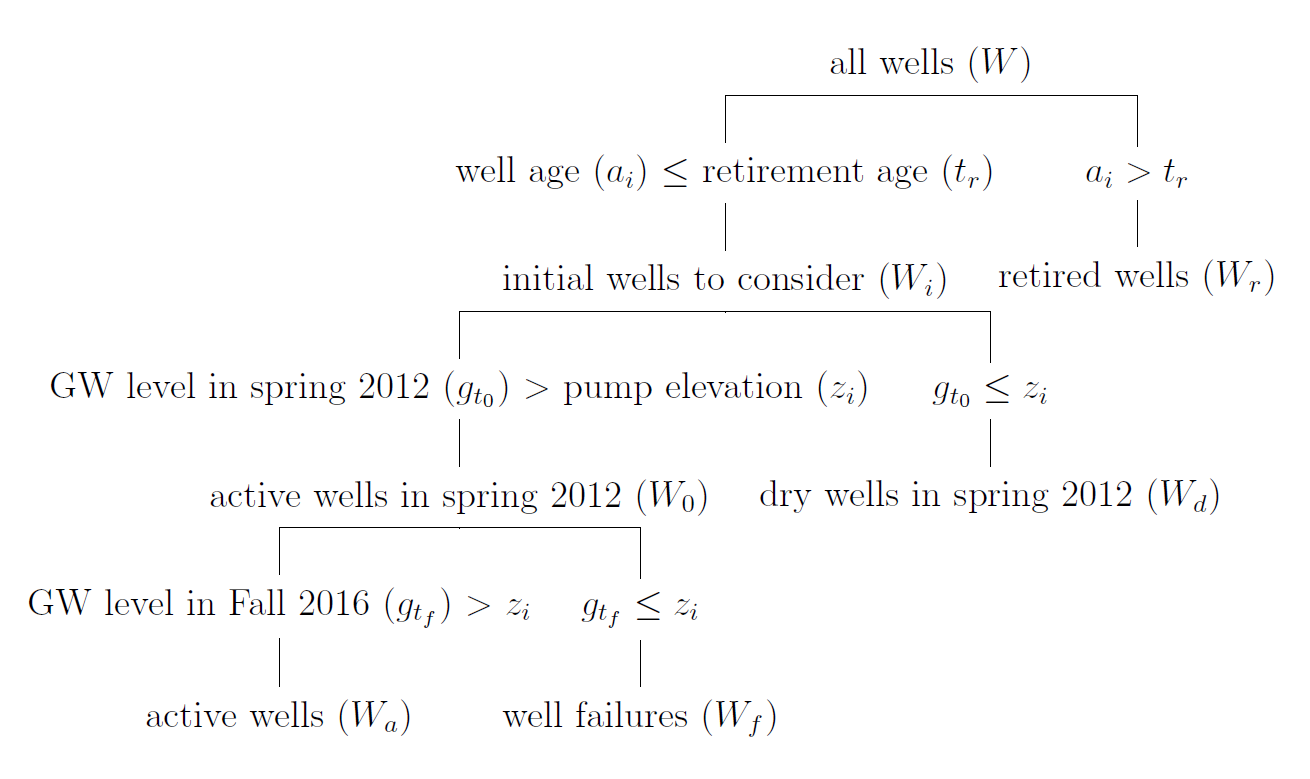
\includegraphics[width=17.8 cm]{appendix_figs/tree.png}
	\caption{Decision tree representing the steps taken to evaluate active and retired wells, initially active and well failures, and finally, active wells and well failures given the following boundary conditions: retirement age, initial groundwater level, and final groundwater level.}
	\label{fig:tree}
\end{figure}

Classification into active and failing wells proceeds as follows. Let the set of all domestic WCRs be called $W$. First, wells with age $a$ greater than or equal to the calibrated retirement age $t_r$ (Section \ref{ap_a_calib})
 are removed from the simulation. 
%(see section \ref{ss_2_6} for a discussion of how this parameter is determined). 
This yields two sets: the initial wells to consider ($W_i$), and the retired wells ($W_r$).  

$$W_i \subseteq W : a_i \leq t_r$$  

$$W_r \subseteq W : a_i > t_r$$  

The remaining active wells at this point are the initial wells to consider, $W_i$. However a well may not be active at $t_0$ frame if its pump is above the groundwater level at $t_0$. Next, wells with pumps above the groundwater level at the start of the simulation were removed, yielding another two sets: the active wells at time zero $W_a(t_0)$, and the failing wells at time zero $W_d(t_0)$. 

The active wells at time zero are the subset of initial wells to consider where the groundwater level at time zero $g({t_0})$ at the location of the well exceeds the pump depth $z$, and the failing wells at time zero are the wells where the groundwater level at time zero at the location of the well falls at or below the pump depth.  

$$W_a(t_0) \subseteq W_i : g({t_0}) > z$$  

$$W_d(t_0) \subseteq W_i : g({t_0}) \leq z$$

Lastly, the groundwater level field at the final time $g({t_f})$ is applied, yielding the final two sets of wells: well failures $W_d(t_f)$ and active wells $W_a(t_f)$. Well failures are the subset of wells where the final groundwater level at the location of the well falls at or below the level of the pump, and active wells are the subset of wells where the final groundwater level at the location of the well does not fall below the level of the pump.  

$$W_a(t_f) \subseteq W_0 : g({t_f}) > z$$  

$$W_d(t_f) \subseteq W_0 : g({t_f}) \leq z$$  

$W_d(t_f)$ and $W_a(t_f)$ combined form the set of all active wells at time zero $W_a(t_0)$. 

Taken together, the three steps taken to classify wells into active and failing wells are visualized as a decision tree in Figure \ref{fig:tree}.  


%%%%%%%%%%%%%%%%%%%%%%%%%%%%%%%%
\subsection{Vulnerable wells}
\label{ap_a_vi}

Vulnerable wells are defined as wells that may experience a loss in function due to sufficiently low water levels above the estimated pump intake depth. We estimate that 3 $m$ is the threshold at which a well may experience losses in function, based on a pumping rate of 1 $m^3 / hr$, a required net positive suction head of 5 $m$, a barometric pressure head of 10 $m$ (at 25 degrees C and 0 $m$ above mean sea level), a vapor pressure (at 25 degrees C) of 0.3 $m$, and friction head losses of 1 $m$ \cite{Tullis1989}. 


%%%%%%%%%%%%%%%%%%%%%%%%%%%%%%%%
\subsection{Groundwater level interpolation}
\label{ap_a_gwl}

The groundwater level interpolation consists of five steps: (i) data collection; (ii) log transformation; (iii) ordinary kriging; and (iv) back-transformation and correction of the interpolated groundwater levels.  
Groundwater level data covering fall and spring measurements between 1998 and 2017 were obtained from DWR \cite{gwl}. Seasons are defined as either spring (January - March) or fall (August - October). Groundwater levels in a season reflect the ambient signal of the unconfined to semi-confined aquifer. Groundwater levels are measured in reference to the land surface at the measurement locations.

Many environmental data follow a log-normal distribution \cite{Stedinger1980}, including the ambient groundwater levels used in this study. Depths to groundwater at each monitoring well were log transformed ($ln(x)$) prior to interpolation to normalize the data distribution, suppress outliers, and improve data stationarity \cite{DeutschC.V.andJournel1992, Varouchakis2012}. 

Ordinary kriging was then used to interpolate groundwater levels for each season. Inverse distance weighting and thin plate splines were also considered, but discarded because they produced unrealistic groundwater levels near the study area's boundaries, where conditioning data was sparse, and unlike kriging, are susceptible to bulls-eye patterns (concentric areas of equal value around known data points).  
%The interpolation techniques used in this study are well documented (e.g. \cite{JournelA.G.Huijbregts1978}) and beyond the scope of this paper. 
Ordinary kriging parameters were determined by fitting an exponential semi-variogram model. 

Since the expected value of back-transformed log-normal kriging estimates is biased (i.e. - not equal to the sample mean), we apply a correction \cite{Laurent1963, JournelA.G.Huijbregts1978}:  

\begin{equation}
    g = k_0 \cdot exp \Big[ ln(\hat{g}_{OK}) + \frac{\sigma^2_{OK}}{2} \Big]
\end{equation}

Where $g$ is the corrected and back-transformed groundwater level, $\hat{g}_{OK}$ is the ordinary kriging estimate, $\sigma^2_{OK}$ is the kriging variance, and $k_0$ is the correction factor, proportional to the ratio of the mean of the sample values to the mean of the back-transformed kriging estimates.  

Lastly, the the 5 and 95\% confidence intervals of the kriging estimate was determined via: $\hat{g}_{OK} \pm (1.96 \cdot \sqrt{(\sigma^2_{OK})})$. These confidence intervals are propagated through the model to account for uncertainty in the estimated groundwater level.   


%%%%%%%%%%%%%%%%%%% GW levels
\subsection{Impact of drought on seasonal groundwater levels}
\label{ap_a_drought_impact}

Interpolated seasonal groundwater levels in the study area during the 2012-2016 drought exhibit oscillating seasonal variation between spring and fall, a downward trend as the drought progresses from spring 2012 to fall 2015, and an upward trend beginning in spring 2016 and continuing into 2017. Seasonal groundwater level oscillation is a byproduct of agricultural groundwater demand, which peaks during summer and fall months. 

% gw_boxplot_sp_fall in `02_interpolate_all_seasons_GF.Rmd`
% sp_fa_gwl in `06_calibartion_herve_alvar_graham.Rmd`
% sp_fa_gwl.ai in code/00_figures/sp_fa_gwl/pnas_sp_fall_gwl.ai
\begin{figure}[ht]%[tbhp]
	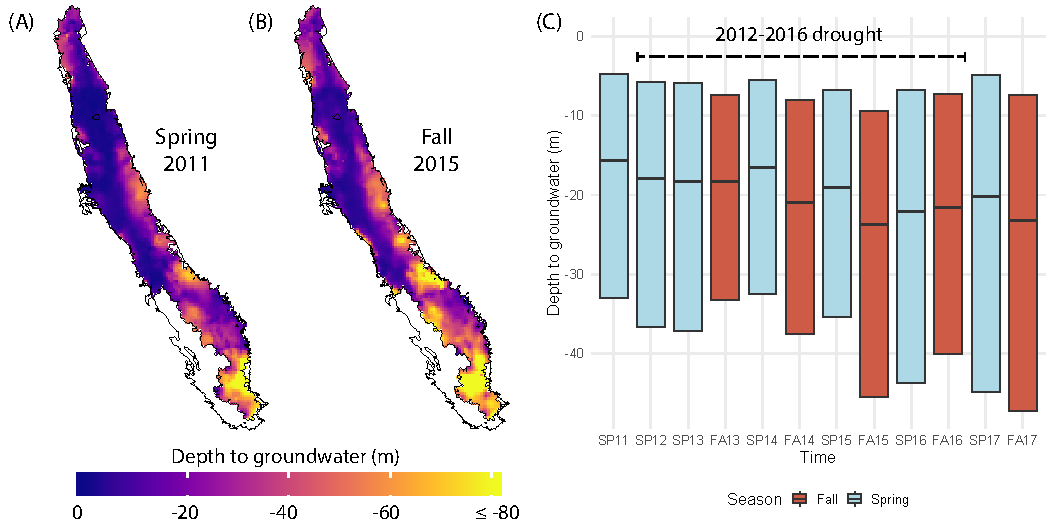
\includegraphics[width=17.8 cm]{appendix_figs/erl_sp_fa_gwl.pdf}
	\caption{Groundwater levels during the most intense 4-year period of the 2012-2016 drought in (A) spring 2011, and (B) fall 2015. (C) Box plots showing the median and 25\% and 75\% percentiles of depth to groundwater. Compared to spring groundwater levels, fall levels tend to be deeper. The schematic assumes that groundwater levels do not decrease with depth, which is not a concern for most of the domestic wells because they tend not to be very deep.}
	\label{fig:sp_fall_gwl_2}
\end{figure}

The median groundwater level oscillates with the growing season (Figure \ref{fig:sp_fall_gwl_2}C) and is generally higher in spring than in fall of the same year. Between spring and fall of 2015 alone, the median groundwater level across the CV fell by nearly 5 $m$. In that same water year, Sierra snowpack measured at an all time low of 5\% of the average snowpack \cite{cadwr2017}, implying that low snowpack leads to more groundwater pumping and hence a seasonal lowering of groundwater levels. 

Median groundwater levels decline between spring 2012 and fall 2015, the four driest consecutive years on California's record (Figure \ref{fig:sp_fall_gwl_2}C). These groundwater level declines coincide with more pumping, which is due to less surface water delivered, which is due to less snowpack. In 2015, California set state records for high temperature, low precipitation, and low snowpack \cite{cadwr2017}. Median groundwater levels start trending upwards in spring 2016 and into 2017, indicating the easing of groundwater pumping. This inflection coincides with the relative return of the Sierra snowpack: in the 2016 and 2017 water years, Sierra snowpack was 85\% and 159\% of normal \cite{cadwr2016, cadwr2017}.  

Over the course of the drought, groundwater levels decline most evidently in the southern CV (i.e. - Madera, Kings, Kaweah, Tule, Tulare Lake, and Kern Bulletin 118 subbasins). These findings are consistent with former research indicating that the central and southern CV experienced the largest surface water loss and groundwater replacement in 2016 \cite{Medellin-azuara2016}, and estimates that California replaced more than 70\% of lost surface water supply with groundwater during the 2012-2016 drought \cite{Lund2018}. 


%%%%%%%%%%%%%%%%%%%%%%%%%%%%%%%%
\subsection{Pump intake depth estimation}
\label{ap_a_pump_depth}


The depth of the pump intake in each domestic well, henceforth called the pump depth ($z$), was estimated for all wells ($W$) as the mean of the static water level at the time of well completion, and the top of the screened interval. This assumption is based on the fact that well pumps are submerged upon installation, and the mean of the static water level at the time of well completion and top of the screened interval represents an unbiased best estimate of where the pump was likely to be placed. Pump depth could not be directly calculated for wells missing either the static water level or the top of the screened interval. Moreover, pump depth exhibits spatial variance due to geologic heterogeneity and historical groundwater use (Figure \ref{fig:pump_loc_density}), which suggests the need for imputation as a function of spatial location. Thus, simple linear models were developed for all wells located within a Bulletin 118 subbasin relating the logarithm of pump depth $z$ to the logarithm of screen bottom, $z_{b}$ (Figures \ref{fig:pump_loc_bottom}-\ref{fig:north_south_impute}). 

\begin{equation}
  log(z) = \beta_{0} + \beta_{1}log(z_{b}) + \epsilon
\end{equation}

Conveniently, $z_{b}$ is known for nearly all wells in the study area. Where it was unknown, it was taken as the total completed depth. Linear models for each subbasin were used to impute the pump depth for wells missing either static water level, top of screened interval, or both.  

%% Distribution of pump depth in B118 SB for data-dense basins (n > 75)
%% pump_loc_density.pdf in `08_pump_loc_spatially_varying.Rmd`
\begin{figure}
	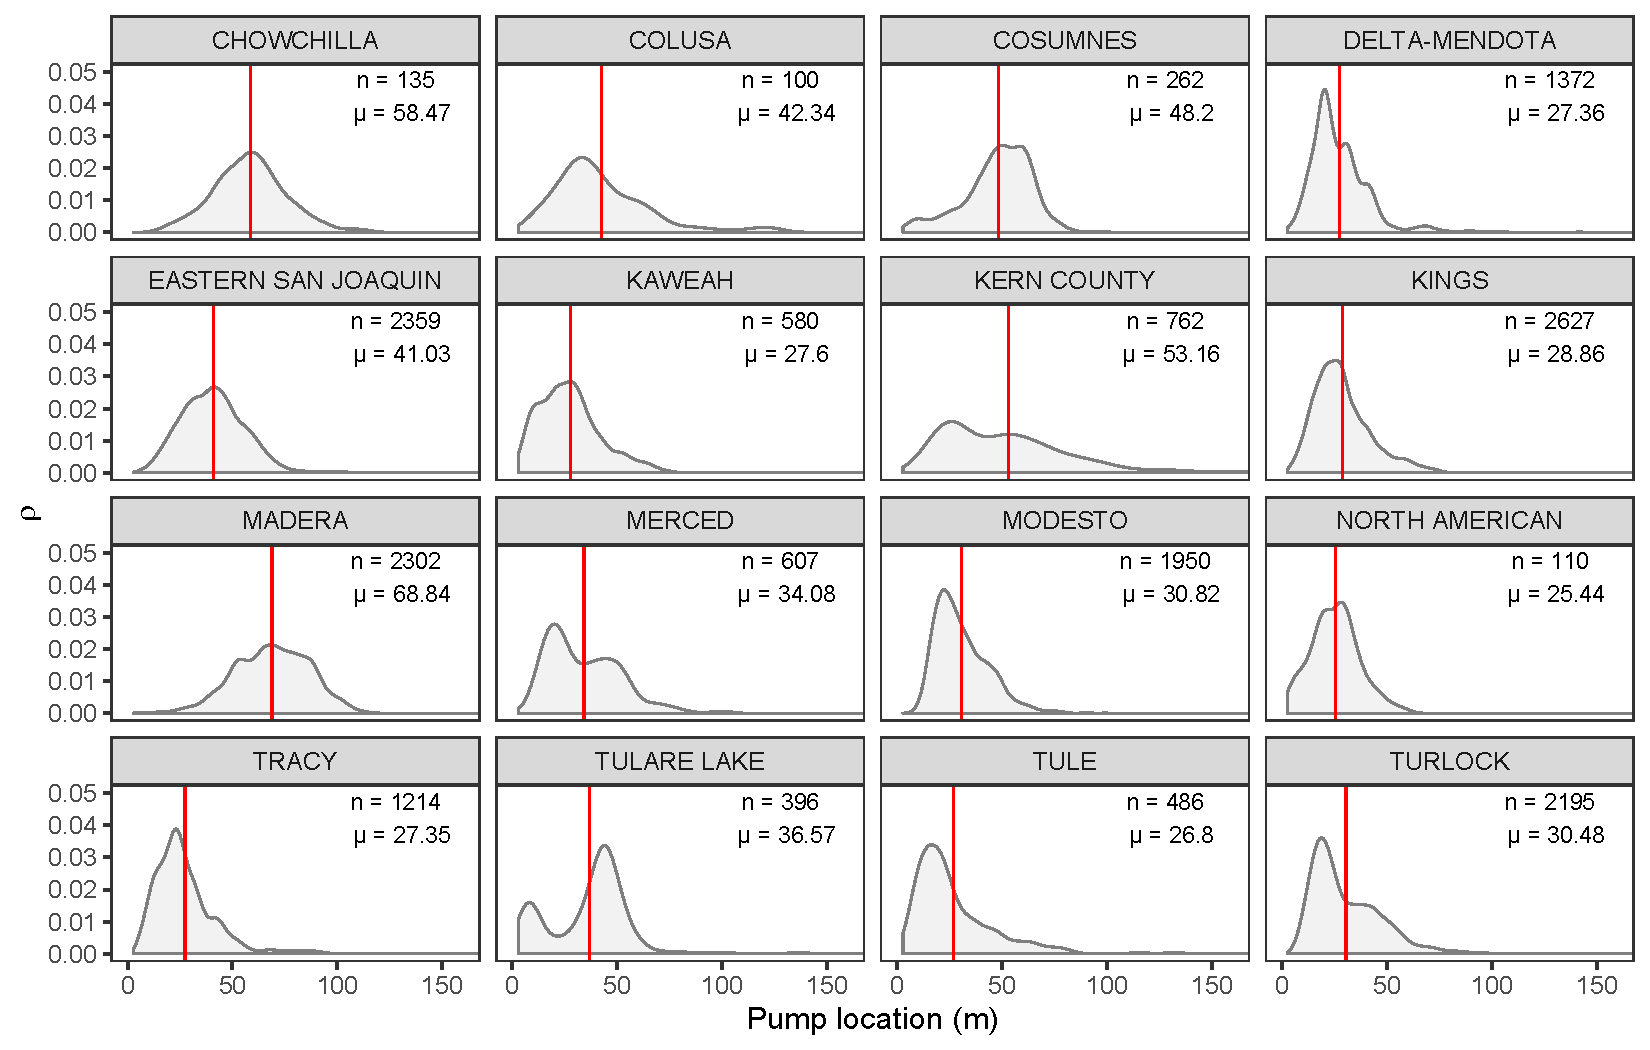
\includegraphics[width=\textwidth]{appendix_figs/erl_pump_loc_density.pdf}
	\caption{Density distributions of estimated pump intake depth for a subset of 16 Bulletin 118 subbasins. The red vertical line indicates the mean pump depth.}
	\label{fig:pump_loc_density}
\end{figure}

% linear model data clouds and line of best fit
%% p_pump_loc_bot.pdf in `08_pump_loc_spatially_varying.Rmd`
% touched up in code/00_figures/pump_loc_bot/ ... ai
\begin{figure}[ht]
	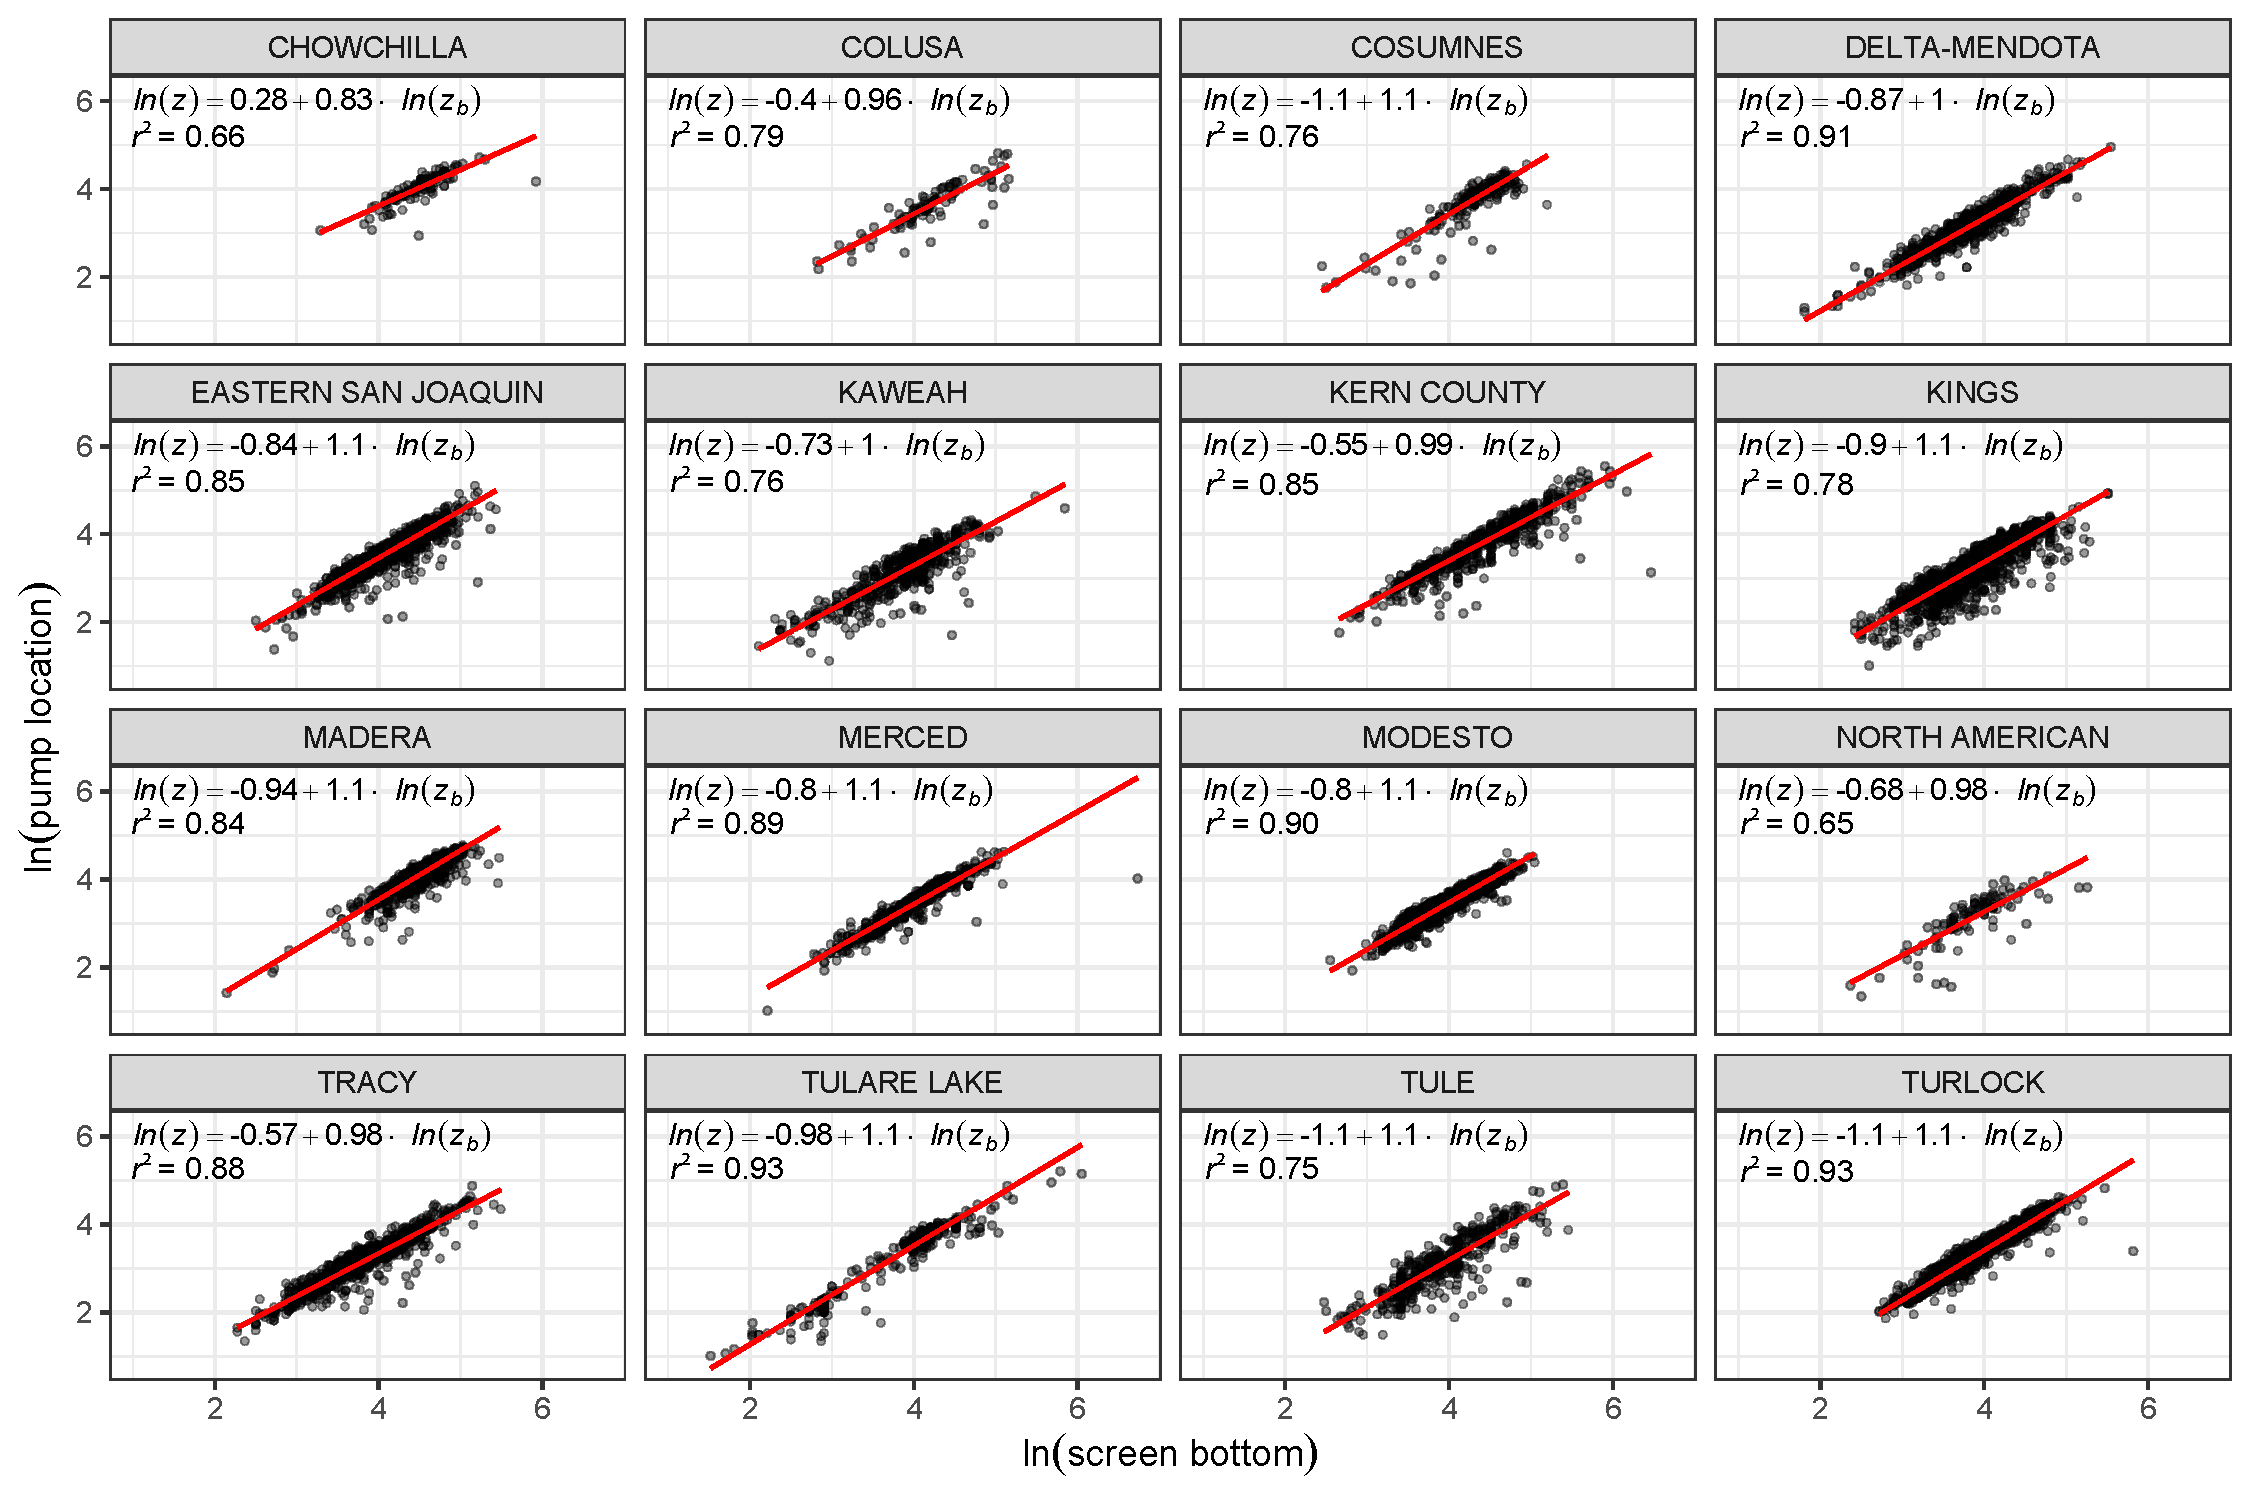
\includegraphics[width=\textwidth]{appendix_figs/erl_pump_loc_bot_eq.pdf}
	\caption{Relationship between the logarithm of pump depth ($z$), and logarithm of the bottom of the screened interval ($z_{b}$) for a subset of 16 Bulletin 118 subbasins.}
	\label{fig:pump_loc_bottom}
\end{figure}

% map of data dense basins, data poor basins, SBs used to construct linear models, and lines of best fit
%% north_south_impute.png in `08_pump_loc_spatailly_varying.Rmd`
\begin{figure}[ht]
	\includegraphics[width=\textwidth]{appendix_figs/erl_north_south_impute_eq.pdf}
	\caption{(A) Count of wells per Bulletin 118 subbasin with recorded screen bottom and directly estimable pump depth, further classified into northern and southern subbasins. (B) \& (C) Northern and Southern subbasins used to construct the linear relationships between pump depth and screened interval bottom; the wells within are shown as black points. (D) \& (E) Northern and Southern linear models used to impute pump depth for northern and southern basins with fewer than 75 samples.}
	\label{fig:north_south_impute}
\end{figure}

Pump depth estimates were generally poor in Bulletin 118 subbasins with fewer than 75 wells, such as in the western San Joaquin Valley, and in various subbasins from the Sacramento Valley to the northernmost CV (Figure \ref{fig:north_south_impute}A). To improve pump depth estimates in these regions, we used observations from adjacent subbasins (Figures \ref{fig:north_south_impute}B \&  \ref{fig:north_south_impute}C) to construct linear models relating pump depth and screen depth as described above (Figures \ref{fig:north_south_impute}D \&  \ref{fig:north_south_impute}E).  

The 5 and 95\% confidence intervals for each linear model were calculated via the standard approach \cite{james2013introduction}, and propagated through the model to account for uncertainty in the estimated pump location.   


Distributions of estimated pump intake depth at the DWR Bulletin 118 subbasin level tend to be either normal or left-skewed (Figure \ref{fig:pump_loc_density}), indicating that most pumps are shallow and close to the land surface. The mean estimated pump depth across subbasins ranges from 25.44 $m$ in the North American subbasin to 68.84 $m$ in the Madera subbasin, suggesting that many pumps are, within tens of meters of the land surface. Considering that most groundwater levels are also tens of meters below land surface %(Figure \ref{fig:sp_fall_gwl_2})
, the distance between a particular well's pump and the upper groundwater level may be only a few meters. Consequently, small groundwater level declines of only a few meters during a drought can lead to considerable domestic well failures.  

The strong relationship between the bottom of the screened interval and the estimated pump depth (Figure \ref{fig:pump_loc_bottom}) was a useful approach for imputing missing pump depths. Goodness of fit ($r^2$) for subbasins have a median of 0.84, and range from 0.93 to 0.41. Residual plots were examined and do not exhibit non-constant variance in the error terms or heteroscedasticity, partially because log-transformation dampens the leverage of the few particularly deep wells. Model $\beta_1$ coefficients vary around 1, indicating that in most subbasins, an increase of 1 unit in the screened interval depth corresponds to an increase of 1 unit in the estimated pump depth. As expected, most intercepts ($\beta_0$) are negative, because the bottom of the screened interval is always deeper than the pump depth. Those with positive intercepts (Yolo and Chowchilla) have poor $r^2$ scores compared to other subbasins, attributable partly to a relatively low number of wells.  

Northern basins are smaller in area than southern basins, and also tend to be more sparse in terms of screened interval information. The sparsity of data in some basins motivated the creation of north and south aggregate models (Figures \ref{fig:north_south_impute}A-E) to supplement data-poor basins with fewer than 75 samples. The south and north aggregate models show an $r^2$ of 0.90 and 0.71 respectively. 

Model coefficients, goodness of fit scores, and sample sizes are reported in Table \ref{tab:linear_mod_coef}.


%% Table of linear model coefficients for SBs and north/south aggretate models
% pl_lm.rds and ns_lm.rds in `08_pump_loc_spatially_varying.Rmd`
\begin{table}[ht]
	\centering\footnotesize
	\caption{Linear regression model coefficients, goodness of fit, and sample size for the subset of wells with 75 or more samples.}
	\label{tab:linear_mod_coef}
	\begin{threeparttable}
		
		\begin{tabular}{lcccr}
			\hline
			\hline
			$Subbasin \: Name$ & $\beta_0$ & $\beta_1$ & $r^2$ & $n$ \\
			\hline
			Chowchilla & 0.28 & 0.83 & 0.66 & 133 \\ 
			Colusa & -0.40 & 0.96 & 0.79 &  98 \\ 
			Cosumnes & -1.06 & 1.12 & 0.76 & 260 \\ 
			Delta-Mendota & -0.87 & 1.05 & 0.91 & 1370 \\ 
			Eastern San Joaquin & -0.84 & 1.07 & 0.85 & 2357 \\ 
			Kaweah & -0.73 & 1.00 & 0.76 & 578 \\ 
			Kern & -0.55 & 0.99 & 0.85 & 760 \\ 
			Kings & -0.90 & 1.06 & 0.78 & 2625 \\ 
			Madera & -0.94 & 1.12 & 0.84 & 2300 \\ 
			Merced & -0.80 & 1.06 & 0.89 & 605 \\ 
			Modesto & -0.80 & 1.07 & 0.90 & 1948 \\ 
			North American & -0.68 & 0.98 & 0.65 & 108 \\ 
			Solano & -0.47 & 0.89 & 0.66 &  75 \\ 
			Tracy & -0.57 & 0.98 & 0.88 & 1212 \\ 
			Tulare Lake & -0.98 & 1.12 & 0.93 & 394 \\ 
			Tule & -1.08 & 1.07 & 0.75 & 484 \\ 
			Turlock & -1.13 & 1.13 & 0.93 & 2193 \\ 
			Yolo & 0.80 & 0.65 & 0.41 &  75 \\ 
			North aggregate & -0.97 & 1.06 & 0.71 & 866 \\ 
			South aggregate & -1.11 & 1.09 & 0.90 & 1920 \\ 
			\hline
		\end{tabular}
		
		\begin{tablenotes}[para,flushleft] 
			Logarithm of pump depth $z$ is regressed onto the logarithm of screen bottom elevation, $z_{b}$.
		\end{tablenotes}
	\end{threeparttable}
	
\end{table}



%%%%%%%%%%%%%%%%%%%%%%%%%%%%%%%%
\subsection{Model calibration and performance}
\label{ap_a_calib}

We seek a well failure model that reproduces the observed well failures during 2012-2016 by relating changes in groundwater level to estimated pump locations of wells in the OSWCR database. The developed model may then be used to simulate the impact of future droughts. We perform calibration to minimize error between the observed ($n \! = \! 2,027$) and predicted well failures during the 2012-2016 drought. Model calibration proceeded in three steps. First, groundwater levels across the CV during the 2012-2016 drought were mapped. Second, the spatial units at which the model was calibrated were selected (discussed below). Third, the optimum value of the well retirement age ($t_r$) was determined.

Groundwater levels across the CV were mapped by the interpolation approach described above and in the methods of the paper. In order to calculate groundwater level change over the drought, we set initial and final conditions, and take their difference. Because the observations are not spatially consistent across seasons, we take the mean groundwater level of adjacent seasons to reduce variance in the interpolated surface, and provide a more robust representation of groundwater levels during that time. The initial groundwater level ($g_{t_0}$) is the mean of spring 2011 and spring 2012 measurements, and the final groundwater level is the mean of spring and fall of 2016. The difference of the final and initial conditions defines the groundwater level change over four years of drought from 2012-2016. The upper and lower 2.5 percentiles of the raster (which incidentally coincide with areas of low to zero domestic well occurrence) were assigned to the 2.5 and 97.5 percentiles to control for outliers in the interpolation and improve mapping. The well failure model described in section \ref{ap:22} was then applied.  

%% p_calib_err.png in `06_calibration_herve_alvar_graham_calib_TS.Rmd`
%% GF edit in same file ^^
%% obtain using `lGF_CI.rds` for gw levels with CIs and 
%% `domcv6_mean_gwl_with_beta_GF_CI.rds` for max_gwl during 2012-2016
%% with CIs
\begin{figure}[ht]
	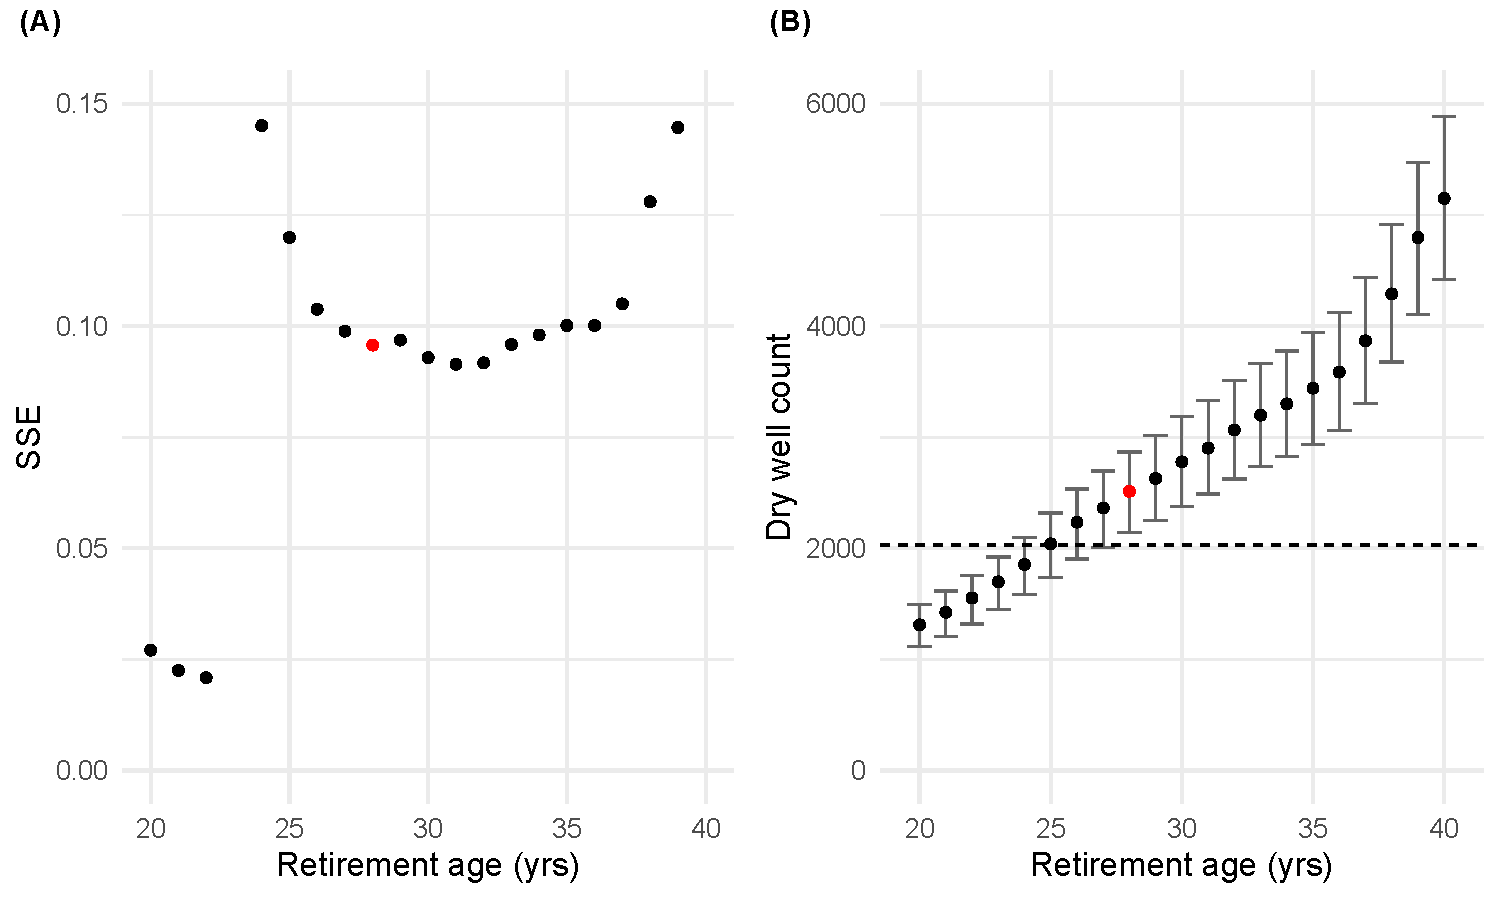
\includegraphics[width=\textwidth]{appendix_figs/erl_p_calib_err_GF.pdf}
	\caption{(A) Retirement age of domestic wells and associated SSE in the calibration spatial units. Low retirement ages remove too many wells from the model, resulting in unrealistically low SSE compared to a validation set. (B) Retirement age of domestic wells and associated count of failing wells during the 2012-2016 drought. The horizontal dashed black line shows the number of observed failing wells during the drought, constraining the feasible solution space to retirement ages of 25 years or greater. The red dot indicates the most reasonable model that balances low SSE, acceptable retirement age (28 years), and a compensation for well failure under-reporting. Error bars show the 5 and 95\% confidence intervals of predicted well failures, computed by propagating uncertainty in pump location estimation and groundwater level estimation through the model.}
	\label{fig:calib_err}
\end{figure}

One free parameter, the well retirement age ($t_r$) controls the number of wells active at time zero and thus the accuracy of the model. The optimum retirement age was determined by minimizing the sum of squared error (SSE) between the observed and predicted proportion of well failure across all calibration units (Figure \ref{fig:calib_err}). Retirement ages from 20 to 40 years were tested, with the assumption that the true retirement age was within this range. SSE is calculated for the observed well failure \textit{proportion} rather than the observed well failure \textit{count}, because proportions are normalized by the total number of wells in each spatial unit. Thus, the error term weights all calibration units equally, and the calibration units with unusually low or high well counts do not exert excessive leverage.  


Three-by-three blocks of PLSS townships (henceforth called aggregate-townships; length = 28.97 $km$, area = 839.16 $km^2$) were selected as the spatial units for calibration for two main reasons. First, since well failure reporting occurs at a county-level, calibration units must be at least this size, which the aggregate-township level achieves. Second, townships are meaningful units of spatial organization to planners and managers. We experimented with smaller calibration scales, such as the PLSS section (length = 1.61 $km$, area = 2.59 $km^2$), and PLSS township (length = 9.67 $km$, area = 93.24 $km^2$). However, small calibration spatial units suffer from high variance in prediction error: some spatial units show very low prediction error (e.g.- zero observed and zero predicted failures), while others show very high prediction error (e.g. - when a large difference between observed and predicted well failures exists). These differences are attributable to uncertainty in well failure reporting, well completion reporting, and groundwater level. A coarser calibration resolution at the aggregate-township (length = 28.97 $km$, area = 839.16 $km^2$) is less likely to contain spatial units with zero observations, and also averages the variance of observed failures at a larger scale, thus permitting spatially-explicit model validation at a coarser resolution. Small spatial units along the alluvial boundary edge less than 600 $km^2$ were removed in order to focus the calibration in regions representative of high well density. 

To further control for uncertainty in the voluntary well failure reporting data, which we expect is more likely to be under-reported than not, only calibration units with observed failure ratios between the 25\% and 95\% percentiles were considered. Like well failure reporting, OSWCR reporting is also likely to under-count total domestic wells, thus only calibration units with well counts between the 25\% and 95\% percentiles were considered. Lastly, only aggregate-townships with at least 20 observed well failures were considered in the calibration. We select this threshold because it represents approximately 1\% of the roughly 2,000 observed well failures during the 2012-2016 drought. Eleven final aggregate-townships were selected to perform the calibration.    


The well retirement age parameter ($t_r = 28$ years) led to the most reasonable model that balanced low SSE, and agreed with the mean retirement age for domestic wells in the CV found by \cite{Gailey2019}. The 2,027 observed failures during the 2012-2016 drought imposes a hard constraint on feasible retirement ages equal to or greater than 25 years, because under this value, the predicted well failure count is less than the observed well failure count (Figure \ref{fig:calib_err}B). Low retirement ages (20-22 yrs) removed too many wells from the model, resulting in unrealistically low well failure count, (Figure \ref{fig:calib_err}A), and high retirement ages (37-40 yrs) left too many wells in the model, which led to high SSE and an unrealistically large number of well failures (greater than observed during the 2012-2016 drought). 

%% calibration_pred_obs_line.ai
%% calib.pdf in `06_calibration_herve_alvar_graham_calib_TS.Rmd`
%% GF edit in ^^ Rmd file and .ai file at calibration_pred_obs_line.ai
\begin{figure}[H]
	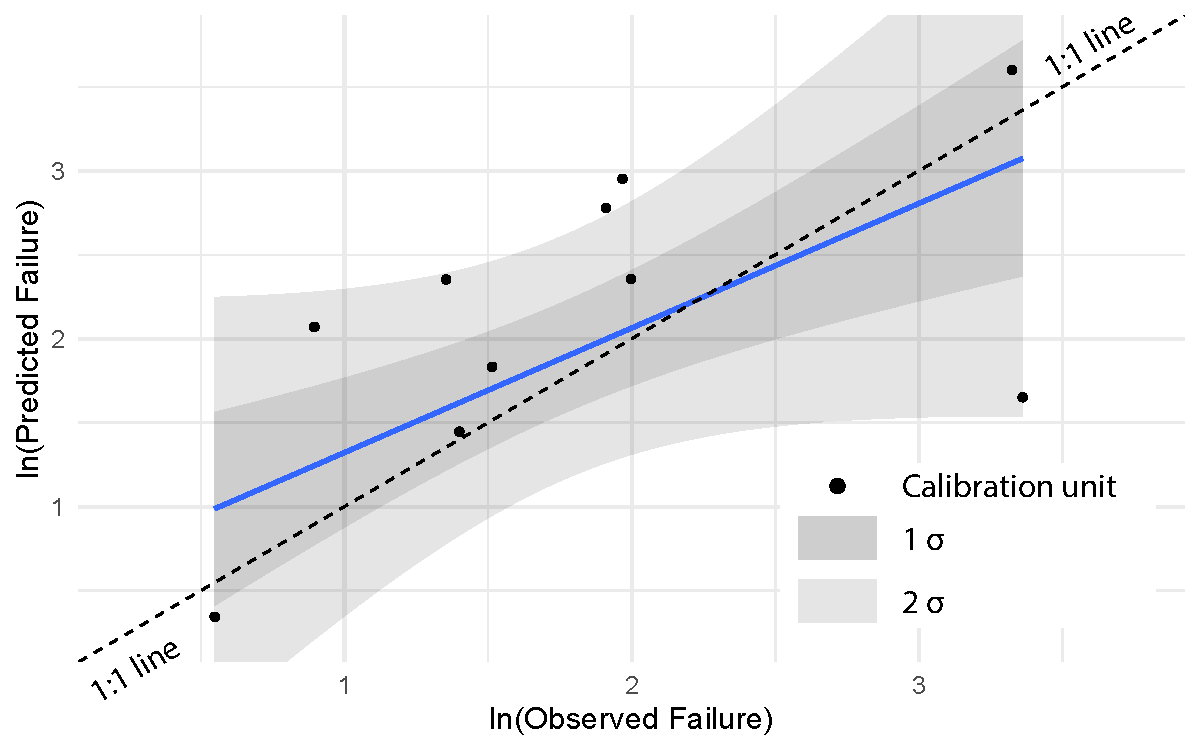
\includegraphics[width=\textwidth]{appendix_figs/erl_calibration_pred_obs_line_GF.pdf}
	\caption{Predicted vs. observed log failure ratio for the 11 calibration spatial units. }
	\label{fig:calib_line}
\end{figure}

The fit between observed and predicted calibration units suggests relatively high local-scale error, with four calibration units falling more than 2 standard deviations from the least squares line through the observed and predicted scatter plot (Figure \ref{fig:calib_line}). These discrepancies are the product of uncertainty in well failure reporting, well completion reporting, groundwater level, and model formulation. As the failure model is subject to local error it is best interpreted as a regional-scale domestic well failure estimate. 

\clearpage

\begin{table}[H]
	\centering\footnotesize
	\caption{Domestic well failure counts under different groundwater management regimes (Sustainable, Glide path, and Business as usual).}
	\begin{threeparttable}
		
		\begin{tabular}{lrrr}
			
			\hline
			\hline
			
			& \textbf{mean failure count} & \textbf{5\% CI failure count} & \textbf{95\% CI failure count} \\
			
			\hline
			
			\multicolumn{4}{l}{\textbf{\textit{Sustainable}}}\\
			\hspace{1em}1998-2017 & 1516 & 1248 & 1809\\
			\hspace{1em}2003-2017 & 2000 & 1619 & 2412\\
			\hspace{1em}2008-2017 & 2513 & 2200 & 2914\\
			
			\hline
			\multicolumn{4}{l}{\textbf{\textit{Glide path}}}\\
			\hspace{1em}1998-2017 & 3677 & 3359 & 4039\\
			\hspace{1em}2003-2017 & 4929 & 4509 & 5361\\
			\hspace{1em}2008-2017 & 6943 & 6501 & 7417\\
			
			\hline
			\multicolumn{4}{l}{\textbf{\textit{Business as usual}}}\\
			\hspace{1em}1998-2017 & 5966 & 5650 & 6293\\
			\hspace{1em}2003-2017 & 7677 & 7239 & 8092\\
			\hspace{1em}2008-2017 & 10466 & 10087 & 10885\\
			\hline
			
		\end{tabular}
		\label{tab:dom_failures}
		\begin{tablenotes}[para,flushleft] 
			The mean failure count corresponds to the number of wells failing when the mean pump depth is used. Well failures at the 5\% confidence interval (CI) and 95\% CI correspond to uncertainty in the estimated pump location. Hydrologic uncertainty in groundwater level is accounted for by considering three different linear approximations of groundwater level decline, beginning in 1998, 2003, and 2008.
		\end{tablenotes}
	\end{threeparttable}
\end{table}

\clearpage



%--------------------------------------------------------%
% Acknowledgements
%--------------------------------------------------------%
\section{Acknowledgments}
We thank the Governor's Office of Planning and Research and the California Department of Water Resources for their assistance in acquiring domestic well failure, and well completion report data. Thomas Harter, Darcy Bostic, and Nisha Marwaha provided modeling advice and assistance. The West Big Data Hub has helped disseminate this research. Financial support was provided by the National Science Foundation (NSF) Climate Change, Water, and Society (CCWAS) Integrated Graduate Education and Research Traineeship (IGERT) program at the University of California, Davis (http://ccwas.ucdavis.edu, DGE-10693333), and the University of California Water (UC Water) Security and Sustainability Research Initiative.


%--------------------------------------------------------%
% Data
%--------------------------------------------------------%
\section{Data availability}
The data that support the findings of this study are openly available. These data\citep{Pauloo2019} do not include observed well failure data \citep{observedDW}, which are confidential and must be obtained by contacting the California Department of Water Resources. 

\clearpage